%%%%%%%%%%%%%%%%%%%%%%%%%%%%%%%%%%%%%%%%%%%%%%%%%%%%%%%%%%%%%%%%%%%%%%%%%%%%%%%%
\chapter{Постановка задачи и выбор средств реализации}
%%%%%%%%%%%%%%%%%%%%%%%%%%%%%%%%%%%%%%%%%%%%%%%%%%%%%%%%%%%%%%%%%%%%%%%%%%%%%%%%

В данном разделе производится постановка задач, которые решаются в ходе работы над диссертацией, их описание, а также рассматриваются требования и ограничения, стоящие при их выполнении.

%%%%%%%%%%%%%%%%%%%%%%%%%%%%%%%%%%%%%%%%%%%%%%%%%%%%%%%%%%%%%%%%%%%%%%%%%%%%%%%%
\section{Задача инструментирования исходных текстов программ}
%%%%%%%%%%%%%%%%%%%%%%%%%%%%%%%%%%%%%%%%%%%%%%%%%%%%%%%%%%%%%%%%%%%%%%%%%%%%%%%%

Как уже было рассмотрено ранее, под инструментированием \textit{обычно} понимают возможность отслеживания параметров программного обеспечения посредством встраивания дополнительного (инструментирующего) кода в исследуемое ПО.

Из этого определения видно, что инструментирование является частным случаем модификации (трансформации) программного кода.
Поскольку все возможные варианты трансформаций состоят из простейших операций, таких как \textit{вставка/добавление}, \textit{замена/обновление} и \textit{удаление}, в данной работе будет рассмотрен процесс инструментирования только с точки зрения \underline{вставки} некоторого, определяемого пользователем, программного кода в исходный текст программы.

Для более общего случая возможен следующий порядок организации выполняемых групп действий:
\begin{enumerate}[noitemsep]
  \item удаление;
  \item обновление;
  \item добавление;
\end{enumerate}
однако, данный порядок может зависеть от решаемой пользователем задачи, и не является предметом рассмотрения в данной работе.

С учетом этого, целью данной работы является разработка мультиязычной расширяемой программной системы, позволяющей производить автоматическое инструментирование исходного текста программы в соответствии с правилами, задаваемыми пользователем такой системы.
Для достижения поставленной цели необходимо:
\begin{itemize}[noitemsep]
  \item разработать подход к задаче инструментирования:
    \begin{itemize}[noitemsep]
      \item разработать метод обхода конкретного дерева разбора;
      \item разработать подход к реализации контекстов инструментирования;
    \end{itemize}
  \item разработать прототип генератора систем инструментирования исходного текста программ;
  \item убедиться в жизнеспособности разработанного подхода, выполнив инструментирование с помощью разработанного инструмента и проведя анализ файлов из различных проектов с исходными текстами на разных ЯП;
\end{itemize}

%%%%%%%%%%%%%%%%%%%%%%%%%%%%%%%%%%%%%%
\subsection{Требования к разрабатываемому подходу}
%%%%%%%%%%%%%%%%%%%%%%%%%%%%%%%%%%%%%%

Сформулируем основные требования к разрабатываемому генератору систем инструментирования для решения первой задачи:
\begin{itemize}[noitemsep]
  \item должен позволять проводить инструментирование исходных текстов программ, созданных с помощью различных языков программирования;
  \item должен быть рассчитан на совместимость с ЯП, использующими императивное и структурное программирование;
  \item должен позволять пользователям самостоятельно описывать необходимые контексты инструментирования;
  \item должен иметь возможность инструментирования основных управляющих конструкций выбранного пользователем языка программирования.
\end{itemize}

%%%%%%%%%%%%%%%%%%%%%%%%%%%%%%%%%%%%%%
\subsection{Требования к прототипу}
%%%%%%%%%%%%%%%%%%%%%%%%%%%%%%%%%%%%%%

Сформулируем основные требования к разрабатываемому генератору систем инструментирования для решения второй задачи:
\begin{itemize}[noitemsep]
  \item должен реализовывать разрабатываемый подход к решению задачи инструментирования;
  \item должен позволять проводить инструментирование исходных текстов программ, созданных с помощью различных языков программирования;
  \item должен быть рассчитан на совместимость с ЯП, использующими императивное и структурное программирование;
  \item должен позволять пользователям самостоятельно описывать необходимые контексты инструментирования;
  \item следует считать входные файлы с исходным текстом программ и файлы фрагментов синтаксически-корректными;
  \item должен быть кросплатформенным и работать под управлением операционных систем семейств Windows и Linux.
\end{itemize}

%%%%%%%%%%%%%%%%%%%%%%%%%%%%%%%%%%%%%%%%%%%%%%%%%%%%%%%%%%%%%%%%%%%%%%%%%%%%%%%%
\section{Анализ задач и выбор подходов к решению}
%%%%%%%%%%%%%%%%%%%%%%%%%%%%%%%%%%%%%%%%%%%%%%%%%%%%%%%%%%%%%%%%%%%%%%%%%%%%%%%%

%%%%%%%%%%%%%%%%%%%%%%%%%%%%%%%%%%%%%%
\subsection{Выполнение трансформаций текста программ}
%%%%%%%%%%%%%%%%%%%%%%%%%%%%%%%%%%%%%%

Для осуществления трансформаций исходных текстов программ, созданных с помощью широкого спектра различных (императивных) языков программирования, необходимо либо реализовать собственное средство, позволяющее выполнять требуемые преобразования с учетом нюансов отдельно взятых языков программирования, либо использовать существующее средство или язык (с соответствующей средой выполнения) такие как, например, ASF+SDF, Stratego/XT, Rascal, TXL~\cite{cordy2009eating} или подобные им.
\nomenclature{ASF}{Algebraic Specification Formalism.}
\nomenclature{SDF}{Syntax Definition Formalism.}

TXL -- это язык программирования, специально разработанный для поддержки задач анализа компьютерного программного обеспечения и преобразования исходных текстов посредством структурной трансформации на основе правил как парадигмы быстрого решения сложных вычислительных задач.
Язык сочетает в себе элементы функциональных и основанных на правилах языках программирования с унификацией, базирующейся на итерационном  подходе с рекурсивным сопоставлением шаблонов~\cite{txl-about}.

В качестве одной из существующих реализаций среды для исполнения программ на языке TXL выступает утилита FreeTxl (далее -- ``утилита TXL'').
FreeTxl -- это бесплатный компилятор/интерпретатор программ для языка TXL, основанный на применении XML, распространяемый лабораторией университета Куинс в Кингстоне~\cite{txl-freetxl}.
Существенными реимуществами данной утилиты являются~\cite{txl-freetxl}:
\begin{itemize}[noitemsep]
  \item наличие бинарных исполняемых файлов для различных программных платформ и аппаратных платформ;
  \item возможность вывода результатов в виде XML-документа (дерева);
  \item является официальной средой для работы с языком TXL, развиваемой разработчиком самого языка описания трансформаций.
\end{itemize}

Исходя из приведенных выше достоинств, было принято решение об использовании утилиты FreeTxl для выполнения над исходными текстами этапа трансформаций, порождаемых генератором систем инструментирования.

%%%%%%%%%%%%%%%%%%%%%%%%%%%%%%%%%%%%%%
\subsection{Обработка деревьев разбора}
%%%%%%%%%%%%%%%%%%%%%%%%%%%%%%%%%%%%%%

Существуют следующие основные методы обхода древовидных структур данных~\cite{cormen2009introduction}:
\begin{itemize}[noitemsep]
  \item обход в глубину (DFT) -- дерево проходится вниз настолько, насколько это возможно на каждом потомке перед переходом к следующему родственному поддереву;
  \item обход в ширину (BFT) -- посещение каждого узла на одном уровне прежде чем перейти на следующий уровень;
  \item обход методом Монте-Карло -- алгоритм, основывающийся на статистических эвристиках.
\end{itemize}
\nomenclature{DFT}{Depth-First Traversal -- метод обхода графовой структуры, состоящий в том, чтобы идти ``вглубь'' графа, насколько это возможно.}

Утилитой TXL используется алгоритм обхода в глубину~\cite{txl-about}, вследствие чего все требуемые способы обхода деревьев разбора должны базироваться на DFT.
Это означает, что обход производится начиная из вершины с узлом, имеющим тип $program$, спускается на наибольшую возможную глубину (лист) первой ветви дерева, попутно обрабатывая узлы указанного типа, затем продолжая обрабатывать аналогичным образом оставшиеся поддеревья данного.

Приведенные выше рассуждения приводят к формулировке метода, который способен решить поставленную задачу, а именно -- нисходящего однопроходного метода.

%%%%%%%%%%%%%%%%%
\subsubsection{Нисходящий однопроходный метод}
%%%%%%%%%%%%%%%%%

\nomenclature{CST}{Concrete Syntax Tree -- конкретное дерево разбора.}

Основная идея нисходящего подхода заключается в постепенном спуске по дереву разбора, которое генерирует внутри себя утилита TXL, от корневого узла к листьям, сохраняя по пути следования информацию для определения контекста, в котором находятся обрабатываемые узлы и выполняется инструментирование.

Данный метод хорошо соотносится с функциональной природой языка TXL, с помощью которого можно описать цепочку вызовов взаимосвязанных функций для обработки различных вложенных типов узлов дерева разбора.

Однако, данный метод подходит только для таких языков программирования, которые соответствуют принципу вложенности синтаксических элементов, т.е. программы, составленные на данных языках программирования соответствуют \textit{структурной} парадигме программирования~\cite{struct-programming}.

Важно отметить, что из требования вложенности узлов дерева CST, содержащих данные для определения контекста инструментирования, следует, что контекст будет определен верно только при наличии всех данных, требуемых для проверки ограничений, задаваемых при определении контекста.

%%%%%%%%%%%%%%%%%
\subsubsection{Нисходящий многопроходный метод}
%%%%%%%%%%%%%%%%%

Основная идея нисходящего многопроходного метода инструментирования заключается в разделении прохода сбора данных для определения контекста и выполнении инструментирования из нисходящего однопроходного метода на три последовательных этапа.

\underline{Первый} этап, подготовительный, заключается в многократном постепенном спуске по дереву разбора, которое генерирует внутри себя утилита TXL, от одного корневого узла к листьям, с целью сбора и распространения (вниз по дереву) информации, необходимой для определения контекста инструментирования.

\underline{Второй} этап, размечающий, заключается в однократном постепенном спуске по дереву разбора с целью определения принадлежности рассматриваемой точки различным контекстам инструментирования с сохранением результатов этих проверок в виде наборов контекстов, которым соответствует текущий узел CST.

\underline{Третий} этап, заключительный, заключается в однократном постепенном спуске по дереву разбора с целью выполнения инструментирования, основываясь на принадлежности конкретной точки контекстам.

Данный метод требует для своей работы наличия или автоматического создания некоторого типа узла дерева CST, который бы являлся общим для \textit{всех} типов рассматриваемых узлов в соответствии с различными пользовательскими правилами инструментирования.

В данной работе для построения прототипа генератора систем инструментирования исходных текстов программ будет рассмотрено применение только нисходящего однопроходного метода.

%%%%%%%%%%%%%%%%%%%%%%%%%%%%%%%%%%%%%%
\subsection{Контексты инструментирования}
%%%%%%%%%%%%%%%%%%%%%%%%%%%%%%%%%%%%%%

Инструментирование требует определения точного положения рабочей точки, в которой оно должно быть выполнено.
Для этого необходимо определение контекста, в котором оно выполняется.
Следовательно, выполнение инструментирования подразумевает определение и использование некоторых контекстов, в которых оно выполняется или, наоборот, не должно выполняться.
При этом, в данной работе, под контекстом подразумевается некоторое множество точек инструментирования.
Одним из возможных способов задания множеств является формализация множества посредством описания в виде $Y = \{g \in G \mid A(g) \}$, где $A(g)$ -- условие принадлежности элемента $g$ некоторому множеству $Y$.
В данном случае под $G$ следует понимать все множество узлов конкретного дерева разбора.
При этом свойство $A(g) \in \{0, 1\}$ позволяет использовать этот метод для организации множеств операции булевой логики первого порядка.

Однако теперь необходимо решить задачу сопоставления множеств поддеревьям CST с учетом того, что правила грамматики, описанные с помощью возможностей языка TXL, позволяют описывать бесконечные деревья, потому как зачастую образуют графовые структуры, содержащие циклические ссылки.
На рисунке~\ref{fig:tree-inf} показан пример, демонстрирующий два конкретных дерева разбора, правила грамматики которых (выделено фиолетовым) позволяют описывать бесконечные последовательности вида $ABAB ... {C_N}$.

\begin{figure}[!h]
	\centering
	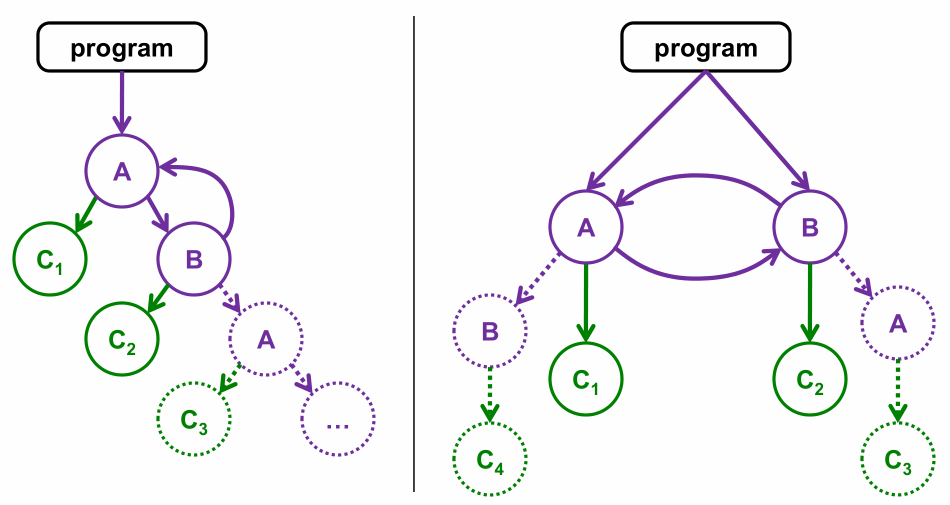
\includegraphics[width=3.2in]{tree_inf}
	\caption{Пример дерева разбора с повторением типов узлов}
	\label{fig:tree-inf}
\end{figure}

Для решения этой задачи рассмотрим пример.

Пусть дано выражение $A(g) * B(g) + C(g) * D(g)$, где $A(g)$, $B(g)$, $C(g)$, $D(g)$ -- функции-ограничения, являющиеся признаками принадлежности некоторого узла $g$ различным контекстам инструментирования.

В языке TXL ключевое слово $where$ используется для описания ограничений при составлении правил трансформаций и функций~\cite{txl-book}.
При этом выражения, стоящие друг за другом объединяются посредством операции конъюнкции.

Перечислим существующие формы записи оператора $where$:
\begin{itemize}[noitemsep]
  \item Без модификаторов -- выражение равносильно операции логической дизъюнкции, т.е. результат будет иметь значение \textit{ложь} тогда и только тогда, когда каждая часть выражения примет значение \textit{ложь}.
  \item Модификатор $all$ -- выражение равносильно операции логической конъюнкции, т.е. результат будет иметь значение \textit{истина} тогда и только тогда, когда каждая часть выражения примет значение \textit{истина}.
  \item Модификатор $not$ -- выражение равносильно отрицанию операции логической конъюнкции, т.е. результат будет иметь значение \textit{истина} тогда и только тогда, когда хотябы одна часть выражения примет значение \textit{ложь}.
  \item Модификатор \textit{not all} -- выражение равносильно отрицанию операции логической дизъюнкции, т.е. результат будет иметь значение \textit{истина} тогда и только тогда, когда каждая часть выражения примет значение \textit{ложь}.
\end{itemize}

Видно, что вариант использования ключевого слова $where$ без модификаторов вместе с правилом объединения последовательно идущих ограничений позволяют выразить любое логическое выражение, стоящее в конъюнктивной нормальной форме (КНФ).
Исходя из этого, выражение $A(g) * B(g) + C(g) * D(g)$ после преобразования в КНФ представляет собой следующую цепочку дизъюнкций, соединенных операцией конъюнкции: $(A(g) + C(g)) * (A(g) + D(g)) * (B(g) + C(g)) * (B(g) + D(g))$.

Далее необходимо распределить перечисленные признаки в соответствии с предложенным ранее подходом к организации обхода дерева разбора -- по функциям в соответствии с узлами из дерева разбора, содержащие в момент выполнения трансформаций значения, которые необходимо проверить для определения контекста инструментирования.

Важно отметить, что язык, который используется для программирования утилиты TXL, принадлежит к семейству функциональных, и это ограничение заставляет передавать собираемые данные узлов дерева разбора одним из следующих способов:
\begin{itemize}[noitemsep]
  \item посредством аргументов/параметров, с которыми вызываются последующие функции в цепочке функций;
  \item с помощью именованных глобальных переменных;
  \item с помощью операций ввода/вывода для синхронной передачи и хранения данных во внешнем вспомогательном ПО.
\end{itemize}

Наиболее предпочтительным с точки зрения времени работы и используемой памяти является передача с помощью аргументов/параметров, с которыми вызываются последующие функции в цепочке.
В данном случае цепочка функций является решением задачи инструментирования с учетом приведенного выше однопроходного метода обхода дерева разбора.
Рассмотрим подробнее обобщение одного элемента такой цепочки функций.

На рисунке~\ref{fig:filter_abstract} приведена абстрактная модель функции фильтрации по контексту инструментирования.
Обозначенный механизм ``scope~lock'' заменяет обозначение ключевого слова $skipping$ языка TXL, позволяющего пропускать вложенные узлы одного выбранного типа.

\begin{figure}[!h]
	\centering
	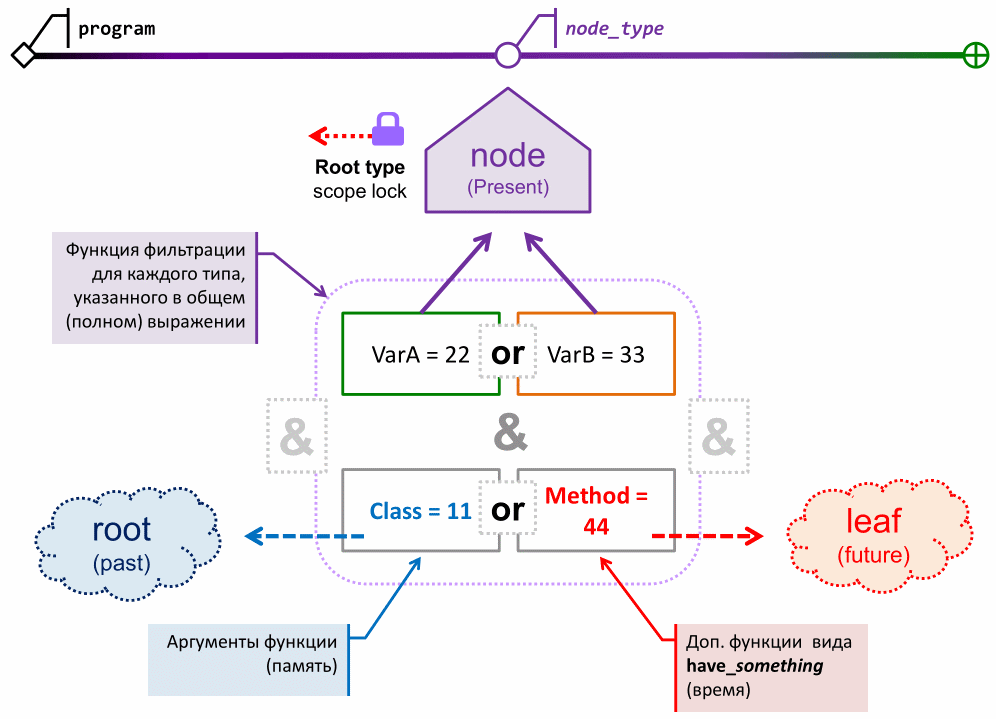
\includegraphics[width=3.5in]{filter_abstract}
	\caption{Модель функции фильтрации по контексту инструментирования.}
	\label{fig:filter_abstract}
\end{figure}

Видно, что для успешного выполнения своих задач рассматриваемая функция ожидает наличия каких-либо заранее заданных источников данных в обрабатываемом узле дерева разбора, и, вместе с тем, каких-то данных, которые не содержатся в текущем узле.

Для решения этой проблемы необходимо рассмотреть различные способы группировки ограничений, объединенных в дизъюнкции.

На рисунке~\ref{fig:filter_types} приведен пример группировки по типам узлов дерева разбора, которые содержат данные, на основе которых выполняется принятие решения о принадлежности к контексту инструментирования. Иными словами -- содержат значения, проверяемые ограничениями из формул, описывающих контексты инструментирования.

\begin{figure}[!h]
	\centering
	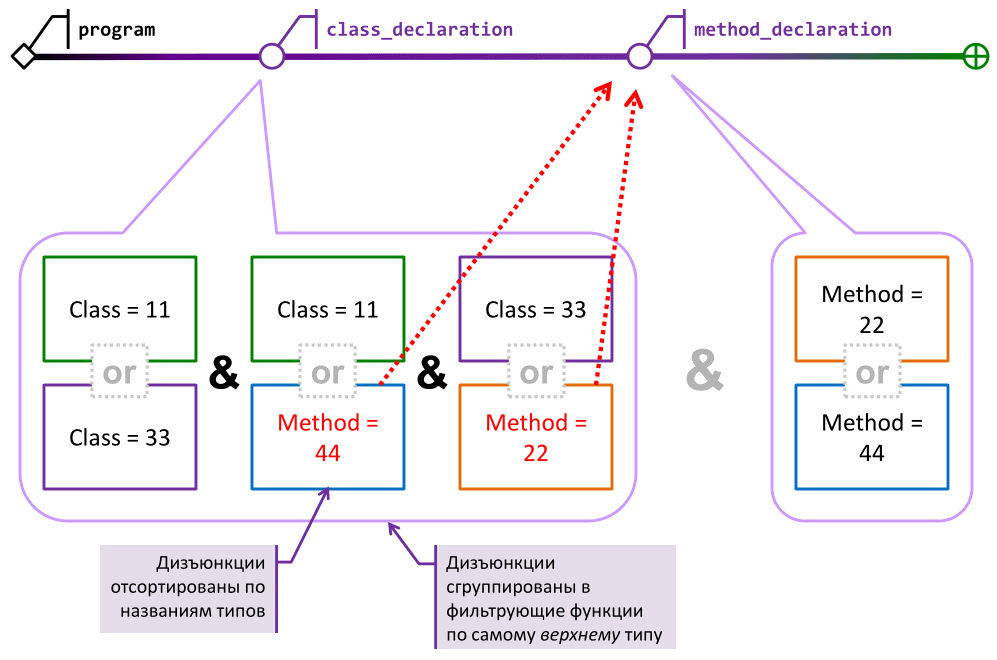
\includegraphics[width=3.2in]{filter_types}
	\caption{Группировка ограничений. Расстановка по типам узлов.}
	\label{fig:filter_types}
\end{figure}

Выражения в дизъюнкциях отсортированы в лексикографическом порядке (по названию элементарного ограничения) и объединены в группы в соответствии с названием самого верхнего элемента.
Для решения возникающей проблемы ограниченной доступности полной информации для определения контекста инструментирования требуется использовать специально подготовленные вспомогательные функции для опроса узлов, находящихся ниже текущего в дереве CST, однако это может лишь сообщить о наличии или отсутствии хотя бы одного узла с требуемыми критериями.
Ошибки возникнут при существовании более одного узла, который удовлетворяет всем критериям поиска.
Вместе с тем, подобный опрос поддерева не позволяет в полной мере управлять процессом спуска по дереву разбора, что усложняет процесс определения принадлежности контексту инструментирования.

На рисунке~\ref{fig:filter_collect} изображен пример, демонстрирующий альтернативный подход группировки с применением специальных дополнительных функций сбора информации с последующей фильтрацией в единой функции проверки принадлежности контексту.

\begin{figure}[!h]
	\centering
	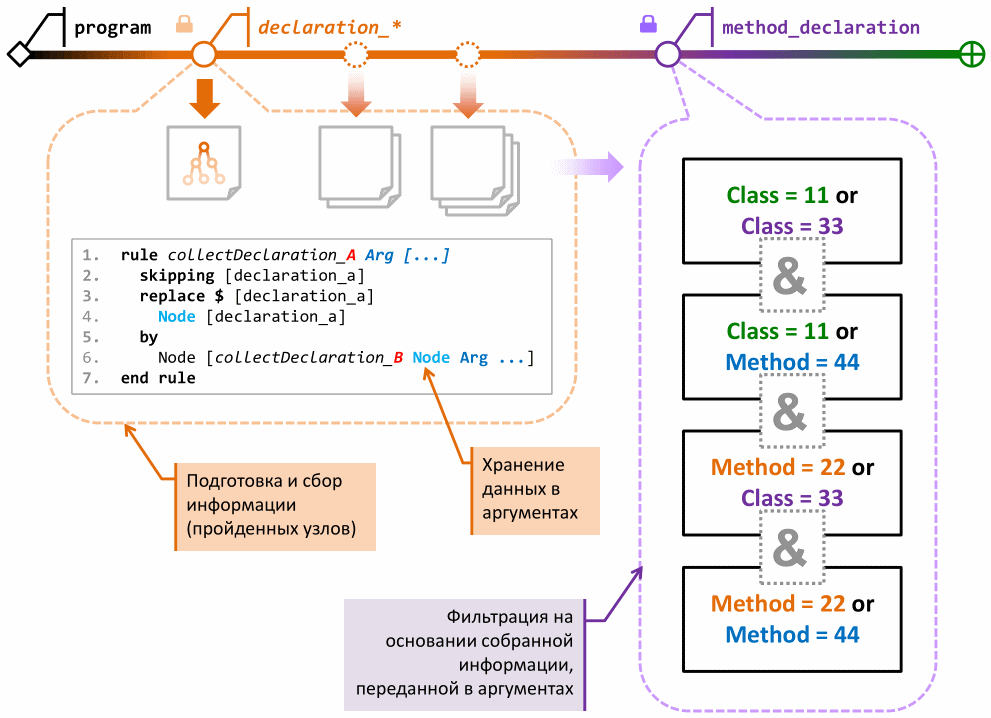
\includegraphics[width=3.7in]{filter_collect}
	\caption{Группировка ограничений. Превентивный сбор информации.}
	\label{fig:filter_collect}
\end{figure}

Подобный подход -- заблаговременный сбор информации, -- позволяет гарантировать точность определения принадлежности узла контексту инструментирования.
Однако, работа метода обхода дерева разбора должна быть учтена при реализации такого подхода, потому как без наложения ограничений, согласно алгоритму работы этого метода, при обработке вложенных структур с одинаковым типом узлов, представляющих эти структуры, возможны пропуски при восстановлении реальной цепочки вложенности из сохраненных в аргументах узлов дерева разбора.

%%%%%%%%%%%%%%%%%%%%%%%%%%%%%%%%%%%%%%
\subsection{Ограничения выбранного подхода}
%%%%%%%%%%%%%%%%%%%%%%%%%%%%%%%%%%%%%%

Ниже собраны основные ограничения приведенных выше подходов и методик:
\begin{itemize}[noitemsep]
  \item только языки программирования, придерживающиеся, но не ограничивающиеся структурной парадигмы программирования;
  \item программа на целевом ЯП представима в виде древовидной структуры;
  \item выполнение только вставки/добавления инструментирующего кода;
  \item используемые контексты инструментирования описываются математическим выражением конечной длины, в терминах теории множеств, используя только операции \textit{пересечения}, \textit{объединения}, \textit{разности} и \textit{дополнения};
  \item потенциальная невозможность работы с ``чистыми функциями'' по причине потенциальной модификации некоторого скрытого глобального состояния добавляемым пользовательским кодом;
  \item определение контекста инструментирования только в условиях полной доступности и соответствующей вложенности узлов CST, содержащих свойства, проверяемые пользовательскими ограничениями.
\end{itemize}

%%%%%%%%%%%%%%%%%%%%%%%%%%%%%%%%%%%%%%%%%%%%%%%%%%%%%%%%%%%%%%%%%%%%%%%%%%%%%%%%
\section{Выводы}
%%%%%%%%%%%%%%%%%%%%%%%%%%%%%%%%%%%%%%%%%%%%%%%%%%%%%%%%%%%%%%%%%%%%%%%%%%%%%%%%

В этом разделе были сформулированы задачи, актуальные для данной магистерской диссертации.
Были выбраны решения и определены требования, которые необходимо учитывать при разработке генератора систем инструментирования исходных текстов программ.
Вместе с тем, были рассмотрены основные ограничения выбранных решений.
